\chapter{Theoretical Background}
\label{cap:Background}



%The aging process exerts profound effects on diverse cognitive domains, including learning abilities. While it is commonly believed that learning becomes more challenging with age, research indicates that older adults are still capable of acquiring new knowledge and skills, albeit with some differences and considerations. Understanding the relationship between aging and learning is crucial for promoting lifelong learning and maintaining cognitive vitality in older individuals. Given the impact of music on the brain, as discussed in Chapter \ref{cap:cognition}, exploring its impact on aging adds an intriguing dimension to the investigation 

\section{Cognitive Aging and Neural Plasticity}

%structural and functional changes in the aging brain, cognitive delice, variablilty in older populations, lifestyle factors influencying cogntive aging
Aging is associated with cognitive changes that can impact learning. These changes include a decline in the executive functions, including processing speed, working memory capacity, inhibition, cognitive flexibility and fluid intelligence \cite{Grady2012, Reuter-Lorenz2010}. In aging brains, both global connectivity (long-range cortical fiver structural connections known as white matter) and functional connectivity (information flow dynamics throughout the whole brains) have been found to be less efficient \cite{Spreng2013}. Cognitive regression correlates with local structural and functional brain modifications, involving reduced gray matter in the prefrontal cortex and hippocampus, along with loss of anterior white matter integrity and functional connectivity. Atrophy in the hippocampus, critical for relational memory, can lead to deterioration in working and long-term memory, as well as a drecrease in abstract thinking. This cognitive decline increases the risk for dementia. However, engaging in cognitive and physical exercise can potentially delay age-related hippocampal atrophy or even increase its size \cite{Erickson2011, Fotuhi2012}. Woodard's 18-month study involving 78 older adults demonstrated that  leisure time physical activity could reduce the risk of cognitive decline \cite{Woodard2012}. Engaging in leisure activities and maintaining an active cognitive lifestyle may generally help prevent cognitive decline \cite{Verghese2003}. While cognitive decline typically starts around age 60, substantial variability exists in the older population \cite{Hedden2004}. 
%concept of neuroplasticity modifying cognitive function, cogntive reserve as buffer againts cogntive decline, interaction genetics, experience, cogntive reserve
Contrary to previous beliefs, research has shown that the adult brain retains a remarkable degree of neuroplasticity even in old age \cite{Altenmuller2020}. Neuroplasticity refers to the brain's ability to reorganize and form new neural connections, allowing the aging brain to adapt and rewise in response to learning experiences. Engaging in learning activities offers numerous benefits for older adults, including cognitive stimulation, social engagement, and personal growth. Neural plasticity mechanisms underpin cognitive plasiticity, with the latter being influenced by education, training, exercise, and diet \cite{Greenwood2010}. While cognitive and neuronal plasticity are preserved over a large range of old age, baseline performance, age and training influence the amout of plasticity \cite{Zinke2014}.
%cogntiive reserve models (neural reserve model and compensatory scaffolding model), frameworks for understanding relationshipt between cognitive engagement and aging
To understand the relationship between cognitive engagement and aging, various model approaches are advocated. Grady offers a model illustrating the diverse dimensions interacting with aging \cite{Grady2012}, while Park and Reuter-Lorenz introduce the Scaffolding Theory of Cognitive Aging (STAC) \cite{Park2009}. The STAC proposes that as individuals age, they develop and rely on cognitive reserve, resulting from compensatory neural and cognitive strategies to maintain cognitive function in the face of age-related changes. This theory posits that older adults tap into their accumulated life experiences and cognitive skills to create scaffolds that support their cognitive abilities, allowing them to overcome challenges and sustain their cognitive performance. These scaffolds involve the strategic use of resources, such as memory aids or alternative cognitive pathways, to compensate for declining cognitive functions. The theory emphasizes the adaptive nature of these compensatory mechanisms, suggesting that they are drawn upon in response to specific cognitive demands and challenges. Overall, the Scaffolding Theory highlights the active and dynamic process through which older adults use their cognitive reserves to navigate cognitive tasks effectively despite the effects of aging. Enhancing scaffolds could be cognitive stimulating leisure activities, such as reading, playing music, and participating in social and physical pursuits. Therapies that rely on everyday activities such as dancing, musical training, or playing chess have been shown to induce a far-reaching transfer of learning due to their variability and complexitiy \cite{Shawn2008, Shawn2014}. Gradually increasing the difficulty of learning activities sustains challenge and intrinsic motivation. Studies indicate a correlation between cognitive reserve and better cognitive performance in adulthood \cite{Panico2022}.
Similar to plasticity, cogntive reserve is influenced by education, occupational activities and leisure pursuits \cite{Nucci2012}. Formal education and potential training courses contribute to cognitive reserve. Working activities also play a predictive role for better cognitive reserve, where the degree of intellectual involvement, personal responsibility, and engagement duration are significant factors. 
While the underlying mechanisms behind cognitive reserve are not yet fully understood, researchers believe that they involve greater neuronal connectivity, the ability to recruit alternative brain networks, and a more efficient use of brain resources when performing cognitive tasks. It's important to note that cognitive reserve doesn't provide absolute protection against cognitive decline or brain diseases, but it can delay the onset of symptoms or reduce the severity of cognitive impairment. Encouraging activities that promote cognitive reserve throughout life can be beneficial for maintaining brain health and improving the quality of life as we age.

 Building cognitive reserve aligns with the concept of lifelong learning, the continuous pursuit of knowledge and skills throughout one's life \cite{Leipold2012}. Lifelong learning encompasses ongoing cognitive stimulation, which is essential for maintaining cogntive function and preventing cognitive decline. It can take various forms, such as formal education, vocational training, hobbies, and self-directed learning. Continously engaging in new learning experiences challenges the brain, promotes neural plasticity, and help preserve memory, attention, and other cogntive abilities \cite{Bangert2010}. Acquiring new skills and knowledge in later life fosters adaptive thinking and problem-solving abilities, enabling older adults to approach novel challenges with a flexible mindset and develop effective strategies for navigating various situations \cite{Greenwood2010}. 

In summary, although there are age-related changes in cognition, older adults are still capable of learning and acquiring new knowledge and skills. By understanding the challenges and implementing effective strategies, promoting lifelong learning can provide cognitive stimulation, personal growth, and social engagement for older individuals. Embracing a proactive approach to learning can contribute to maintaining cognitive vitality and overall well-being throughout the aging process.



\section{Musical Training and Cognitive Benefits}
Music training has long been recognized for its numerous benefits, not only in terms of musical proficiency but also in the impact on the brain and  cognitive processes. This chapter aims to explore the intricate relationship between music, the brain, and cognition, shedding light on the various ways in which music affects our cognitive abilities. By examining empirical studies and theoretical frameworks, this chapter aims to shed light on the potential cognitive benefits of music training and their implications for enhancing overall cognitive functioning.

%Music as complex cogntiive activity: various cogntive domaincs, perception,memory, motor skills and emotional processing, multimodal nature of music traiing potential cogntive beneftis
The mulifaced nature of music engages a spectrum of cogniitve domains, inclusing perception, memory, motor skills, and emotional processing. Active music-making, such as playing an instrument or singing, requieres specific focus and concentration at particular time points \cite{Creech2013}. Music-making is a powerful driver of adaptive brain plasticity, triggering structural and funcional adaptations in response to musical engagement across different life stages, from childhood to late adulthood \cite{Altenmuller2020, Altenmuller2007}. Music's impact extends beyond neurobiology, influencing emotional processes through neurotransmitters like serotonin and dopamine. The experience of joy and reward associated with music-making is intricately tied to activty changes within component of the limbic system. Seinfeld characterizes playing a musical instument as "a complex and motivating activity that comprises the coordination of multiple sensory modalities and motor system in a unique way" \cite{Seinfeld2013}. Learning to play a instrument implies not only motor skills but also the acquisition of skills like musical sightreading and translating notations or musical ideas into movement patterns, such as on a keyboard \cite{Stewart2003}. Musical challenges foster both physical and cognitive engagement, offering opportunities to learn new skills and enhancing existing ones \cite{Creech2013}. Importantly, these challenges are ongoing. The progressive impact of musical training on cognitive brain functions might even extend beyond the field of music processing, with higher levels of musical expertise requiring higher-order cognitive function \cite{Oechslin2013a}.

%studies that demonstrate cogntive advantages of musical engagment across age groups - link betewwen musical training and enhanced cogntive functions
Research hat explored the cognitive benefits of musical training across various age groups. In children, music lessons have been linked to increased IQ scores. These improvements are enduring and independent of childrens's socioeconomic status \cite{Schellenberg2006}. Degé et al. attribute the positive influence of music lessons on intelligence to the enhancement of executive functions, which in turn bolster performance on intelligence tests \cite{Dege2011}. Musical practice has been shown to promote auditory attention and hearing noise in young adults \cite{Strait2011}. Additionally, perceptual-motor skills may profit from musical training \cite{Seinfeld2013}. Adult musicians exhibit more verbal and tonal working memory \cite{Oechslin2013a}, as well as enhanced verbal long-term memory \cite{Chan1998}. Among healthy elderly individuals, musical training hat demonstrated enhancements in executive function, attention, working memory, verbal and visual memory, sensorimotor function and subjective well-being \cite{Seinfeld2013, Bugos2007, Dege2018}.

While numerous studies suggest potential cogntive benefits of musical training, the underlying mechanisms are not yet fully understood. It is important to note that the effect sizes observed are often relatively small. However, there is a positive trend indicating that music training can have a favorable impact on cognitive abilities. 


\section{Musical Engagement in Elderly Adults}
% Cognitive Benefits of Musical Engagement in Elderly Adults (cogntive effects of musical engagment specially in eldery adults - memory, executive functions attention, emotional well-being)

%Musical Engagement in aging
The influence of music on brain functions, particulary in the context of healthy elderly individuals, has been a subject of increasing interest in recent years. This section explores the impact of musical engagement on cognitive, emotional, and physical well-being in older adults, highlighting the transformative power of music and its potential to enhance the qualitiy of life during the aging process.

%significance of musical engagement during aging
Music holds the capacity to evoke emotions and enhance subjective well-being in older adults \cite{Croom2015}. Familiar and personally meaningful music music can trigger nostalgia, evoke positive memories, and create a sense of emotional connectedness \cite{Creech2013}. Studies indicate that music therapy interventions effectively reduce anxiety, depression, and stress, contributing to the emotional well-being of older adults \cite{Guetin2013}. These emotional advantages collectively contribute to an overall improvement in the psychological state of older individuals. 
%positive effects on physical health and functionality
Engaging in musical activities can have positive effects on physical health and functional abilities in older adults. Particpating in activities like playing a musical instrument, singing, and engaging in dance or rhythmic movement can improve motor coordination, balance, gait, and overall physical fitness \cite{Creech2013}. Interventions involving rhythmic auditory stimulation have proven beneficial in enhancing motor rehabilitation for individuals with age-related mobility impairments \cite{Thaut2015}. In the domain of stroke motor rehabilitation, music-based interventions show promise due to their integration of motor training and multimodal stimulation \cite{Grau-Sanchez2020, Altenmuller2020}. 
%Catalyst for social interaction and connection
Furthermore, music serves as a powerful catalyst for social interaction and connection among older adults. Engaging in group music-making activities creates opportunities for social engagement, nurturing a sense of community and belonging. The implementation of music-based interventions in senior living communities or nursing homes encourages social interaction, reduces feelings of isolation, and enhances overall social well-being \cite{Creech2013}.
%sustaining youthful brain function
Resent research proposed that music may play a role in sustaining youthful brain function \cite{Rogenmoser2018}. A comparison of chronological age and  "brain age" among amateur musicians, musicians, and non-musicians revealed that amateur musician exhibited the lowest scores, suggesting a potential age-decelerating effect of music on the brain. However, subsequent studies have not consistently replicated these findings \cite{Matziorinis2023}. It is postulated that musical training and active musical engagement may be linked to a challenge resilience factor, contributing to a form of neurocognitive reserve.
%Musical Activities and Cognitice Function (relationship between specific musical activities and cogntive function, insights into the cognitive processes)
Cross-sectional studies have demonstrated that older adults who engaged with music throughout their lives outperformed their non-engaged counterparts across various cognitive domains, including global cognition, working memory, executive funtions, language, and visuospatial abilities \cite{Hanna-Pladdy2011, Hanna-Pladdy2012}. Trained pianists also exhibit faster neural responses to subtle harmonic changes in expressive music \cite{James2008}. Playing an instrument in older adulthood has even been associated with a reduced likelihood of dementia and cognitive imparment \cite{Balbag2014}. This suggests that lifelong musical engagement could function as a multimodel enrichment strategy, potentially preserveing cognitive and brain health in late life \cite{Bottcher2022}. 
Furhtermore, even for musical novices in older adulthood, musical training has shown promising effects. Learning to read mucial notation over three months induced special effects on visuospatial skills and activation in the fusiform gyrus und superior parietal areas in initially muscially naïve adults \cite{Stewart2003}. A study involving 15 weeks of drumming and singing demonstrated improved verbal and visual memory in eight older women \cite{Dege2018}. Additionally, five weeks of musical training for adult novices led to functional audio-motor coupling in the temporal-frontal regions, indicating brain plasticity \cite{Lappe2008, Bangert2003}. A study involving four months of piano practice observed emhancements in cognitive functions related to attention and executive functions, as well as improvements in some domains of quality of life among 29 healthy older adults \cite{Seinfeld2013}. Following six months of piano lessons, older adults experienced better working memory and executive function compared to control groups  \cite{Bugos2007}. The authors attribute this spefic skill transferability of music learning to the unique mulitmodal nature of learning a musical instrument. In a 16-week programm, 65 healthy older adults improved their working memory and processing speed through piano training or specific computer-assisted cogntive training. The piano group, consisting of 30 participants, additionally demonstrated increased verbal fluency skills, category switching, and general and musical self-efficiancy post-training \cite{Bugos2022}. Another study, although unable to replicate the cognitive findings, revealed in a ten-week piano training programm that the motivation to participate in the lessons (which were group sessions with four participants) significantly influenced the cognitive development of the participants \cite{Macritchie2020}

The impact of music engagement on older adults is substantial, encompassing emotional well-being, physical health, cognitive function, and social interaction. Understanding these effects allows us to recongnize the potential for structured musical instruction to significantly impact the lives of aging individuals. Despite numerous studies demonstrating the impact of music on various cognitive functions in older adults, it is important to notice that particpant groups were often small, leading to potential strong individual differences and factors like the short duration of intervention. Additionally, the specific components of music training, such as instrumental practice or singing, may have differential effects on cognitive aging. Nevertheless, on the whole, music training appears promising as an approach to mitigate age-related cognitive decline and promote healthy aging \cite{Klimova2017}.

\section{Musical Abilities}
Musical abilities are part of the general musicality of humans. The concept of musicality is a complex and multifaceted phenomenon that has intrigued scholars and researchers across various disciplines for centuries \cite{Gembris1987, Pausch2022, Roman-Caballero2018}. Defining musicality precisely and universally presents several challenges due to its subjective nature, and the interdisciplinary perspectives through which it can be examined.  This chapter aims to highlight some of the difficulties encountered in defining musicality and discusses the issue of developing musical abilities. Additionally, different approaches assessing musical abilities pose their own set of complications and are presented.

\subsection{Definition}
In dictionaries, musicality often refers to a combination of musical abilities, acoomplishments, and  knowledge \cite{MerriamWebster}. The Oxford Enlish Dictionary defines musicality as, "the quality or character of being musical; accomplishment or aptitude in music; musical sensibility" \cite{OED}. This concept points to the usual expected musical skills, like considering them "good" or "skilled" musical knowledge. As a construct, musicality encompasses a wide range of abilities and behaviors that can be categorized into different levels \cite{Gembris1987}. Of these, musical abilities constitute one of the most significant domains within musicality. Defining and structuring musical abilities is a complex task, similar to the challenge of defining (musical) intelligence in general. Researchers have explored various theoretical frameworks and approaches to capture the multifaceted nature of musical abilities.
Two prominent perspectives exist in understanding mucial abilities: the concept of a general musical factor and the identification of specific musical domains.\\
One approach draws parallels between musical abilities and Spearman's general intelligence factor \cite{Spearman1904}. Just as general intelligence is believed to underlie various cognitive abilities, some researchers propose the existence of a general musical factor that influences overall musical aptitude \cite{Mackintosh2011}. This general factor is thought to encompass a range of musical skills, such as pitch discrimination, rhythm perception, tonal memory, and melodic perception. Supporters of this view argue that a common underlying factor contributes to an individual's proficiency across different musical domains \cite{Pausch2022}.
In contrast to the concept of a general musical factor, other scholars emphasize the existence of distinct musical domains. This perspective aligns with Thurstone's theory of primary mental abilities, which suggests that intelligence is composed of multiple specific factors \cite{Thurstone1931}. Similarly, researchers propose that musical abilities can be categorized into separate domains, such as pitch, dynmaic, rhythm, timbre, and tonal memory. Each domain is considered to represent a unique set of skills and competencies within the broader realm of musical abilities. This domain-specific view recognizes the diversity and complexity of musical talents and acknowledges that individuals may excel in certain domains while exhibiting average or lower proficiency in others. This approach underlies Gardner's theory of multiple intelligences, which posits that human intelligence is comprised of distinct modalities, including musical intelligence \cite{Gardner2006}. According to Gardner, musical intelligence involves sensitivity to rhythm, pitch, melody, and timbre, as well as the ability to express oneself musically and appreciate different musical forms. This theory suggests that musical abilities are not confined to a single factor, but rather encompass a range of skills and talents.
While the debate between a general musical factor and domain-specific abilities continues, it is important to recognize that musical abilities are multifaceted and can manifest differently in individuals. Some individuals may demonstrate exceptional proficiency in one or more musical domains while showing average or below-average performance in others. Furthermore, cultural and environmental factors can shape the development of musical abilities, leading to variations across individuals and contexts \cite{Pausch2022}.
In summary, musicality encompasses a range of skills, attributes, and sensitivities that go beyond musical performance alone. It includes the ability to perceive, interpret, express, create, collaborate, and critically analyze music. Musicality enriches our engagement with music, whether as performers, composers, improvisers, active listeners, or music enthusiasts, and it plays a vital role in the human experience of this art form. Overall, understanding musical abilities requires a nuanced approach that acknowledges the potential existence of a general musical factor, the presence of specific musical domains, and the influence of cultural and environmental factors. Future research in this field can further contribute to our understanding of the underlying mechanisms and interactions that shape musical aptitude and performance.




\subsection{Measuring Musical Abilities}
\label{cap:musicalabilities}
\minisec{Musicality tests}
There are various approaches and methods used to assess and test musicality, each focusing on different aspects of musical abilities and skills. It is suggested that musical abilities can be measured through different tests that assess various domains of musical abilities \cite{Werner2016}. In addition to assessing performance, which is the most obvious observation when testing musical abilities, aural skill tests can be employed \cite{Harrison2018, MacGregor2019, Harrison2017}. These tests measure an individual's ability to perceive and recognize musical elements, such as pitch, rhythm, melody, and harmony, through listening exercises. Tasks such as melodic dictation, rhythmic dictation, interval recognition, chord identification, and harmonic analysis are often included in aural skills assessments. They evaluate a person's auditory perception, memory, and understanding of music. 
Tests related to musical perception and analysis assess an individual's ability to analyze and interpret musical compositions \cite{Lee2020}. They can involve listening to musical excerpts and answering questions about the structure, style, form, tonality, and expressive elements present in the music. Assessors evaluate critical listening skills and the ability to articulate musical observations. 
Musical aptitude tests aim to assess a person's innate musical abilities and potential \cite{Gordon1968}. These tests explore various dimensions of musicality, including pitch discrimination, rhythm perception, tonal memory, and melodic perception. Musical aptitude tests provide insights into a person's predisposition towards musical activities and learning. 
Some assessments incorporate psychological and cognitive measures to evaluate musicality. These tests may explore factors such as musical intelligence, working memory, attention, executive functions, and emotional responses to music \cite{Mullensiefen2013}. Psychological and cognitive assessments provide a broader understanding of the cognitive and emotional processes underlying musical abilities.
As explained before there are also supporters who speak of one general musicality factor. For that Wing \cite{Wing1961} developed a "Standardized Test of Musical Intelligence" which measures different skills that supposidly form a whole musical factor. On the other hand Seashore \cite{Seashore1919} developed a "Measure of Musical Talent" which computes a mulitfactorial apporoach of relativley independent musical abilities. 
It is important to note that no single test can fully capture the complexity and diversity of musicality. Therefore, a comprehensive assessment of musicality often involves a combination of these approaches, considering multiple facets of musical abilities, skills, knowledge, and experiences.

\minisec{Assessing Musical Performance}
Rating musical performance is a complex task that requieres a delicate balance between objective assessment and subjective interpretation. To explore musical performances several computer-based algorithms for audio analysis are developed \cite{Goebl2014}. As they have shown usable for detecting timing, amplitude and pitch in musical performances, there are still many limitations and technical challenges. Since musical performances involve subjective qualitites, they are challenging for computer algorithms to capture accurately. With human raters who bring own expertise and experience, small nuances and artistic intent can be examined with which algorithms may struggle to comprehend. Especially adapting to beginner performances, which often have mistakes and lack fluency in their playing is challenging for computer algorithms since they are designes to work with established patterns and data. The ability of human raters to appreciate the subjective, expressive, and contextutal elements of music, adapt to different styles and skill levels, and provide nuanced evaluation offers them distinct advantages over computer-based algorithms in assessing musical performance. Still, when assessing musical performance many aspects have to be taken into count. 

\begin{figure}[]
	\centering
	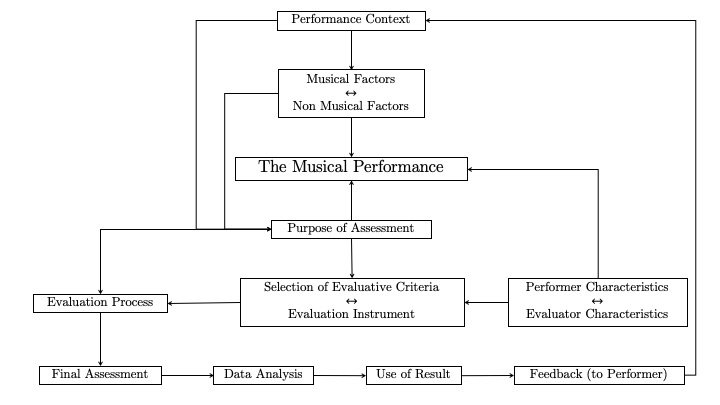
\includegraphics[width=15cm,height=10cm,keepaspectratio]{Assessing}
	\caption{Process Model of Assessing Musical Performance (adapted from \cite{McPhearson1998}))}
	\label{fig:assess}
\end{figure}

McPhearson and Thompson \cite{McPhearson1998} provided a comprehensive summary of the literature regarding the assessment of musical performance, which is depicted in Figure \ref{fig:assess}. To assess "musical performance", various other domains must be considered. Factors such as the "performance context" (e.g., type, purpose, and proportions of the performance) and the "purpose of assessment" (e.g., ranking in competition or research) already influence the evaluation of musical performance. Several musical and non-musical factors can impact the assessment of musical performance. Musical factors, including the choice of repertoire, ensemble size, and expressivity in accordance with the specific composer or period, can affect the rating of a musical performance. Research has demonstrated that non-musical factors, such as the order of appearance, can influence the evaluation of different musical performances \cite{Flores1996}. Listening to various performances of the same piece may result in a greater appreciation of the composition or cause evaluators to begin with higher expectations that gradually adjust to the reality of the performance. Consequently, the characteristics of both the performer and the evaluator are crucial in assessing musical performance. If the performer experiences anxiety or difficulty concentrating during the performance, it significantly impacts the overall quality. Similarly, the personality of the evaluator also plays a significant role. Although research has indicated that training in adjudication does not guarantee better or more consistent evaluation results \cite{Fiske1977}, the evaluator's mood, attitude, and emotional state can influence their assessments. Furthermore, individual listeners' preferences and subjective experiences play a crucial role in the evaluation of musical performance. Musical tastes and preferences vary widely, and what resonates with one listener may not have the same impact on another.  Additionally, the familiarity between the evaluator and performer can substantially impact the evaluation provided. The selection of evaluative criteria is probably the most complex factor for assessing musical performance. To maximise the reliability within the ratings of the evaluators providing a standardised rating scales has proven useful. They establish criteria and guidelines that can be applied uniformly across different performances and context. This constistency allows more reliable comparisons and assessments, enabling performers to track their progress over time. For constructing such scale different criteria are suggested. As first contributor Duerksen provided eight criteria, including rhythmic accuracy, pitch accuracy, tempo, accent, dynamics, tone quality, interpretation, and overall quality \cite{Duerksen1972}. This foundational framework has paved the way for subsequent research. Russell's study devided evaluation criteria into two categories: technical and musical. Technical aspets encompassed tone, intonation, rhythmic accuracy, articulation, and technique, ehile the musical realm involved tempo, dynamics, timbre, interpretaion, and musical expression. Notably, the component of expression had a significant direct effect on the overall perception of quality \cite{Russell2010}. Within institutional frameworkds, the Australian Music Examination Board's Piano syllabus for level 1 underscores accuracy, fluency, rhythmic and metric stability, articulation, dynamics, phrasing, tonal balance, tempo control, and understanding of style and character \cite{AMEB}. The Associated Board of the Royal Schools of Music marking criteria emphasize pitch, time (fluency and rhythm), tone (articulation and dynamics), shape (expressiveness), and overall performance \cite{ABRSM}. Despite the breadth of research and diverse perspectives on performance criteria, a consensus has shown. For evaluation piano beginners' performance the focus lies on technical aspects such as tone and rhythmic accuracy, fluency, articulation, and dynamics, while expressivity complements the components to an overall performance evaulation. \\
In conclusion, the objective rating of musical performance is a complex tast due to the subjectivity of music, the multidimensionality of its elements, the influence of interpretation and artistic choices, contextual considerations, the interplay between technical accuracy and expressive qualities, listener variability, and the limitations of quantitative metrics. While objective measures can provide some insights, a complete evaluation necessitates a balanced approach that incorporates subjective assessments, export judgment, listener feedback, and an appreciation for the artistic an emotional dimensions that make music a captivating and deeply personal form of expression.




\section{Aims/Hypothesis}
musical instrumental prcatice can countervail cognitive and perceptual-motor decline supported by functional and structural brain plasiticity ==> naja, ist nicht mein approach
\\promote healthy mental aging in elderly - independence, autonomy and well-being through musical activities